\documentclass[12pt, a4papre]{article}
\usepackage[catalan]{babel}
\usepackage[unicode]{hyperref}
\usepackage{amsmath}
\usepackage{amssymb}
\usepackage{amsthm}
\usepackage{xifthen}
\usepackage{listings}
\usepackage{float}
\usepackage{siunitx}
\usepackage{graphicx}
\usepackage{indentfirst}

\newcommand{\norm}[1]{\lvert #1 \rvert}
\graphicspath{ {./Images/Memoria2/} }

\hypersetup{
    colorlinks = true,
    linkcolor = blue
}

\author{Daniel Vilardell}
\title{Memoria Practica 2 FISE}
\date{}

\begin{document}
	\maketitle
	
	\tableofcontents
	
	\section{Sessió 1}
	
	Per a aquesta practica s'ha montat i soldat es el seguent.
	
	\begin{figure}[H]
		\begin{center}
		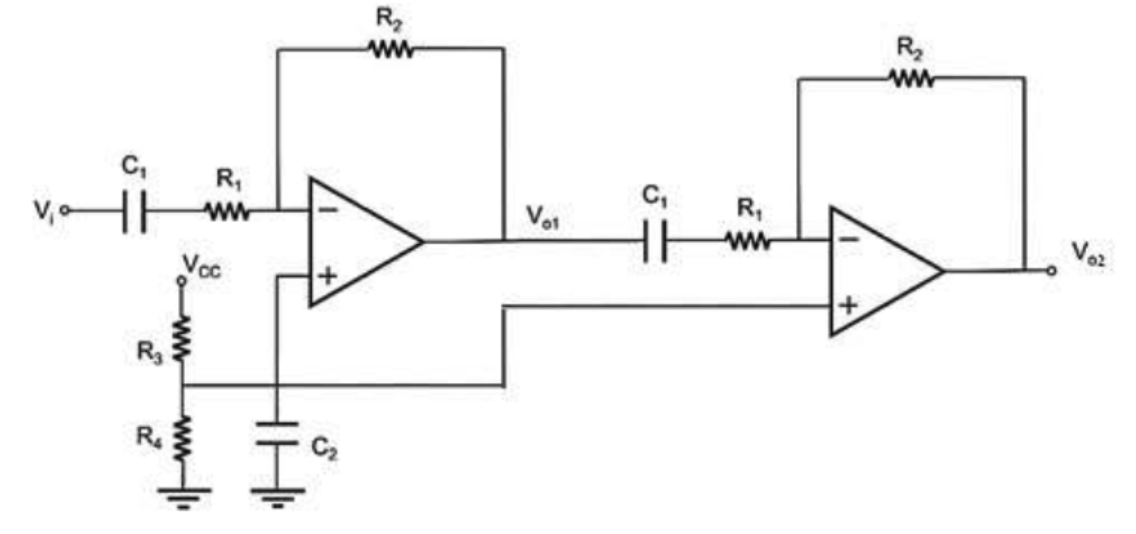
\includegraphics[width=110mm]{previ2_11.png}
		\caption{Circuit practica 2}
		\end{center}
	\end{figure}
	
	En la primera sessió es va montar i comprobar del seu bon funcionament la primera etapa del amplificador, que te la seguent forma.
	
	\begin{figure}[H]
		\begin{center}
		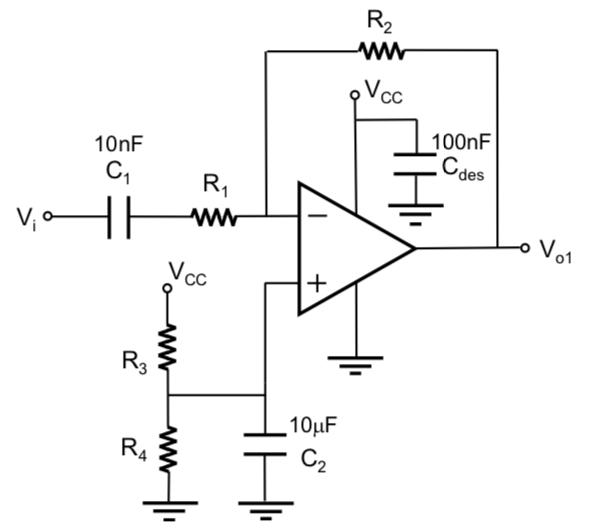
\includegraphics[width=70mm]{img_2_1.png}
		\caption{Primera fase del circuit}
		\end{center}
	\end{figure}
	
	\textbf{Qüestió 1:} La tensió continua mesurada als tres nodes amb continua es la meitat de la alimentació ja que es va agafar $R_3 = R_4$ i per tant la tensió a la pota no inversora del amplificador es de $\frac{V_{cc}}{2}$, que es la mateixa que a la pota inversora gracies al "curtcitcuit virtual" dels amplificadors. Finalment la tensió de sortida del $V_o$ es la mateixa a la pota on inversora ja que el condensador $C_1$ elimina el corrent dins de la conexió entre els nodes, i per tant la corrent no varia.

	\textbf{Qüestió 2:} El senyal a la entrada de la etapa amplificadora es el que posem nosaltres al generador de funcions, que en el nostre cas es una ona a $40kHz$ de $20mV$. A la sortida del amplificador la amplitud de la senyal es de $4V$.
	
	\begin{figure}[H]
		\begin{center}
		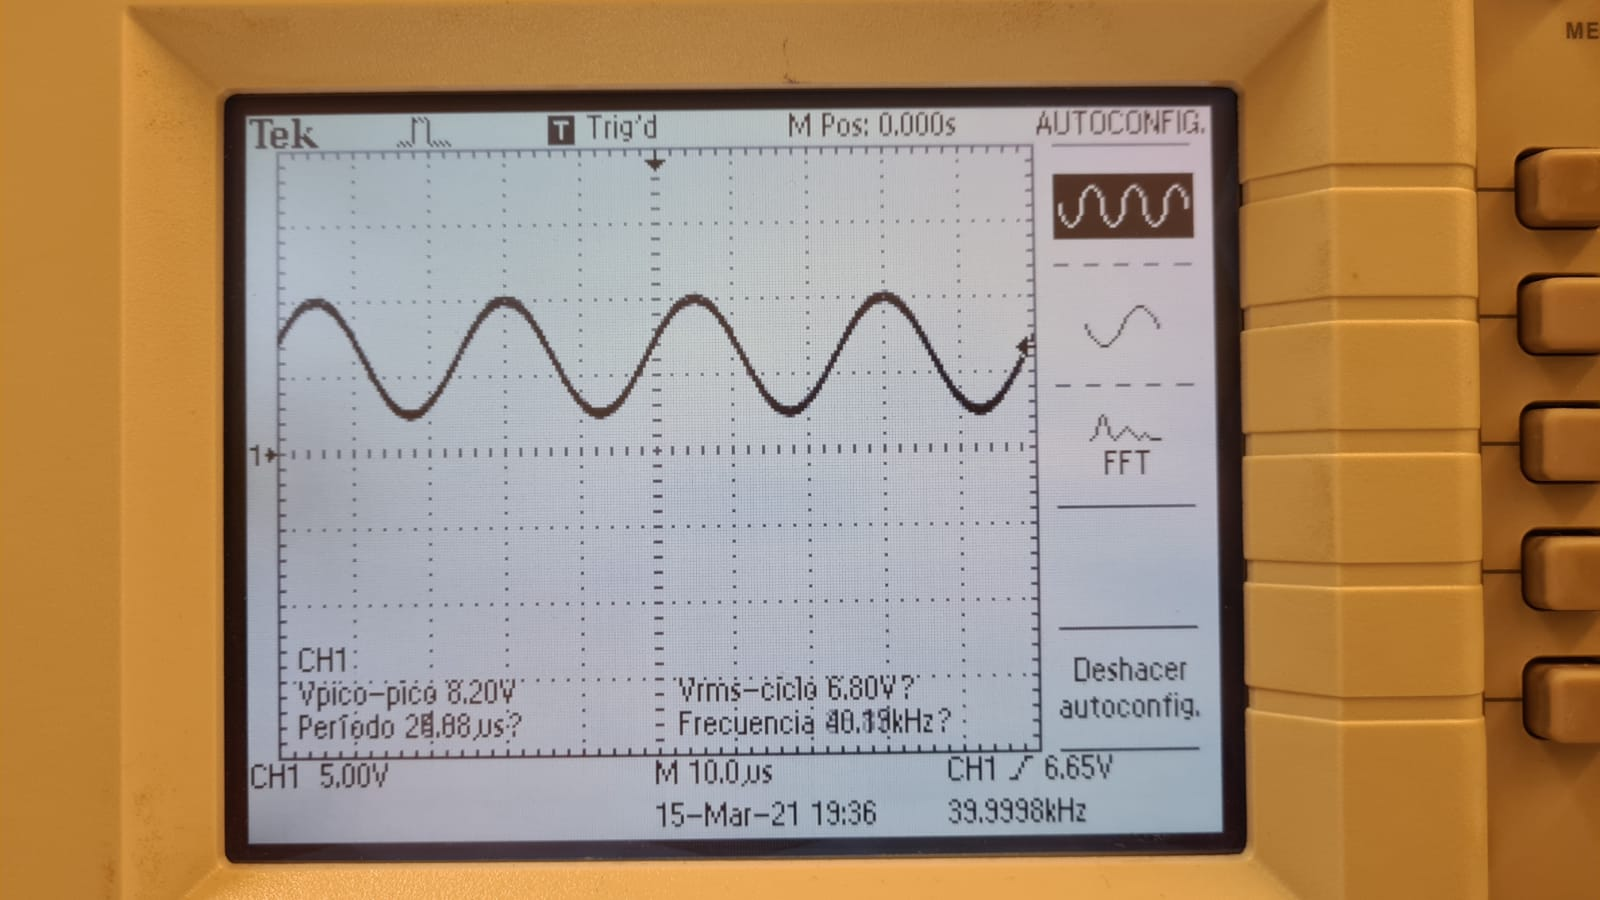
\includegraphics[width=140mm]{img_2_2.jpeg}
		\caption{Sortida per una entrada sinusoidal de $40kHz$}
		\end{center}
	\end{figure}
	
	\textbf{Qüestió 3:}
	
	\begin{center}
		\scriptsize
		\begin{tabular}{ |c|c|c|c|c|c|c|c|c|c| } 
			\hline
			Freqüència & $100Hz$ & $1kHz$ & $10kHz$ & $25kHz$ & $40kHz$ & $75kHz$ & $100kHz$ & $500kHz$ & $1MHz$\\ \hline
			$V_{i1}$ & $20mV$ & $20mV$ & $20mV$ & $20mV$ & $20mV$ & $20mV$ & $20mV$ & $20mV$ & $20mV$\\ \hline
			$V_{o1}$ & $0V$ & $50mV$ & $0.4V$ & $1.7V$ & $4V$ & $1V$ & $0.6$ & $45mV$ & $0$\\ \hline
			Guany & $0$ & $2.5$ & $20$ & $85$ & $200$ & $50$ & $30$ & $2.25$ & $0$\\ \hline
			Guany (dB) & $-$ & $7.9$ & $26$ & $38$ & $46$ & $33$ & $29.5$ & $7$ & $-$\\ \hline
		\end{tabular}
	\end{center}
	
	Al fer la segona etapa es va haver de reduir el quocient $\frac{R_2}{R_1}$ per a evitar que l'amplificació fos tan gran i aixi obtenir la amplificacio de 200 demanada
	
	\section{Sessió 2}
	
	\textbf{Qüestió 4:} Per la mateixa raó que al exericici 1 les tensions mesurades a tots els nodes en continua son $\frac{V_{cc}}{2}$
	
	\textbf{Qüestió 5:} El guany mesurat a cada etapa havent fet els canvis necessaris per fer el quocient $\frac{R_2}{R_1}$ mes petit i tenint una entrada de $10mV$ son:
	
	\begin{itemize}
		\item A la primera etapa la amplificació es de $400mV$ i per tant el guany es de 40.
		\item A la segona etapa el guany es de $4V$ i per tant el guany es de 10.
	\end{itemize}
	El guany total despres de passar per les 2 etapes es de 400.\\\\
	
	\begin{figure}[H]
		\begin{center}
		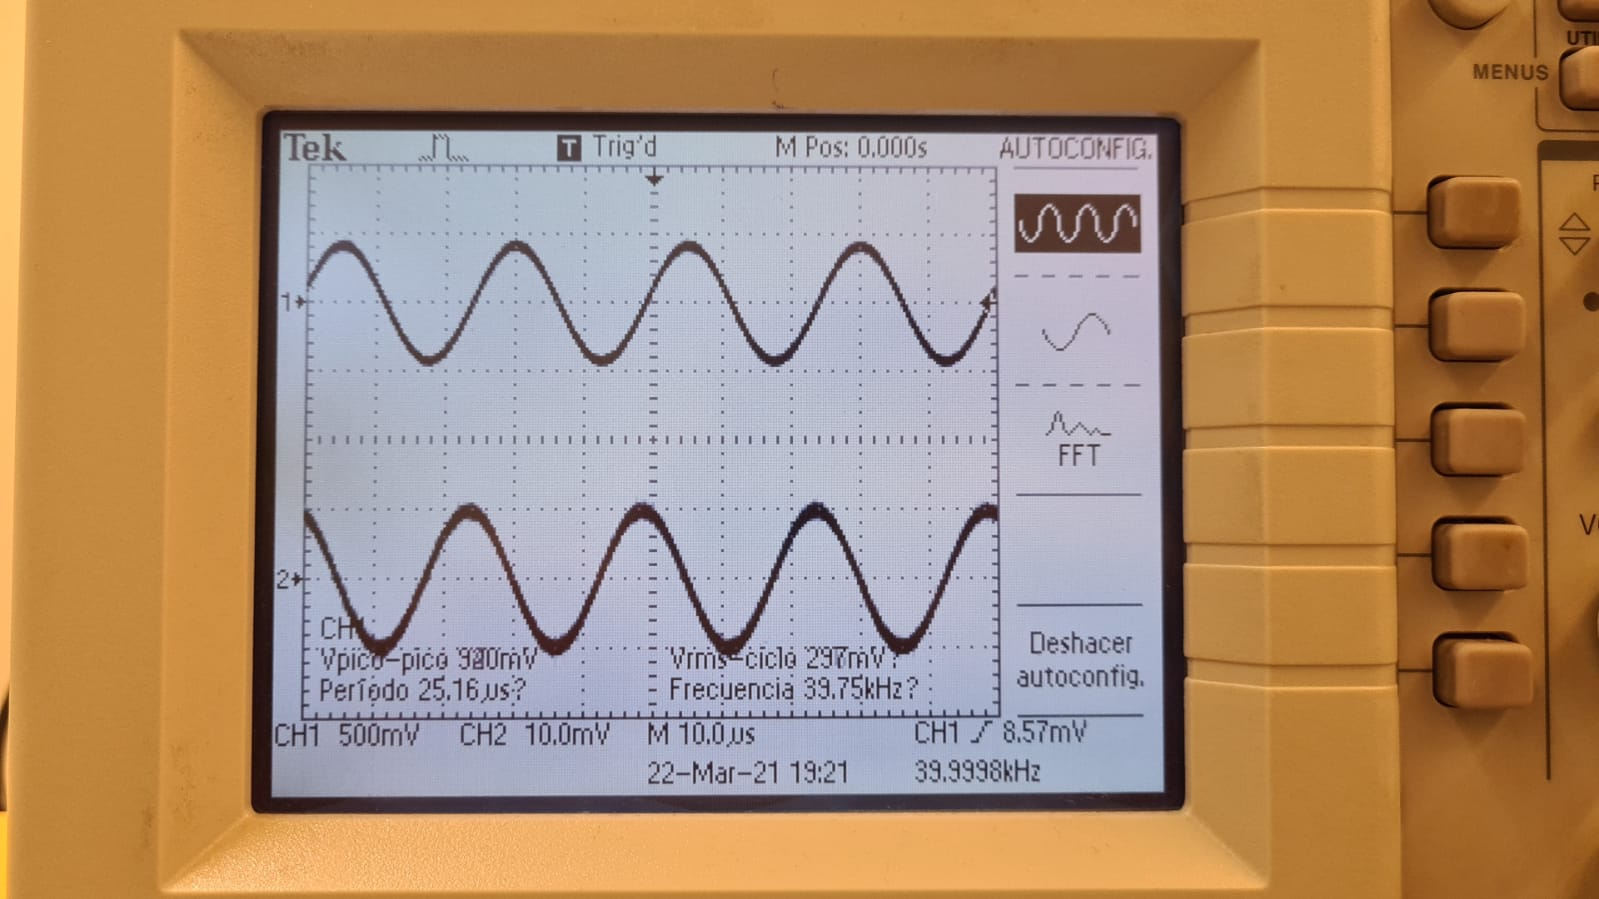
\includegraphics[width=100mm]{img_2_3.jpeg}
		\caption{Entrada i sortida de la primera etapa amplificadora}
		\end{center}
	\end{figure}
	
	\begin{figure}[H]
		\begin{center}
		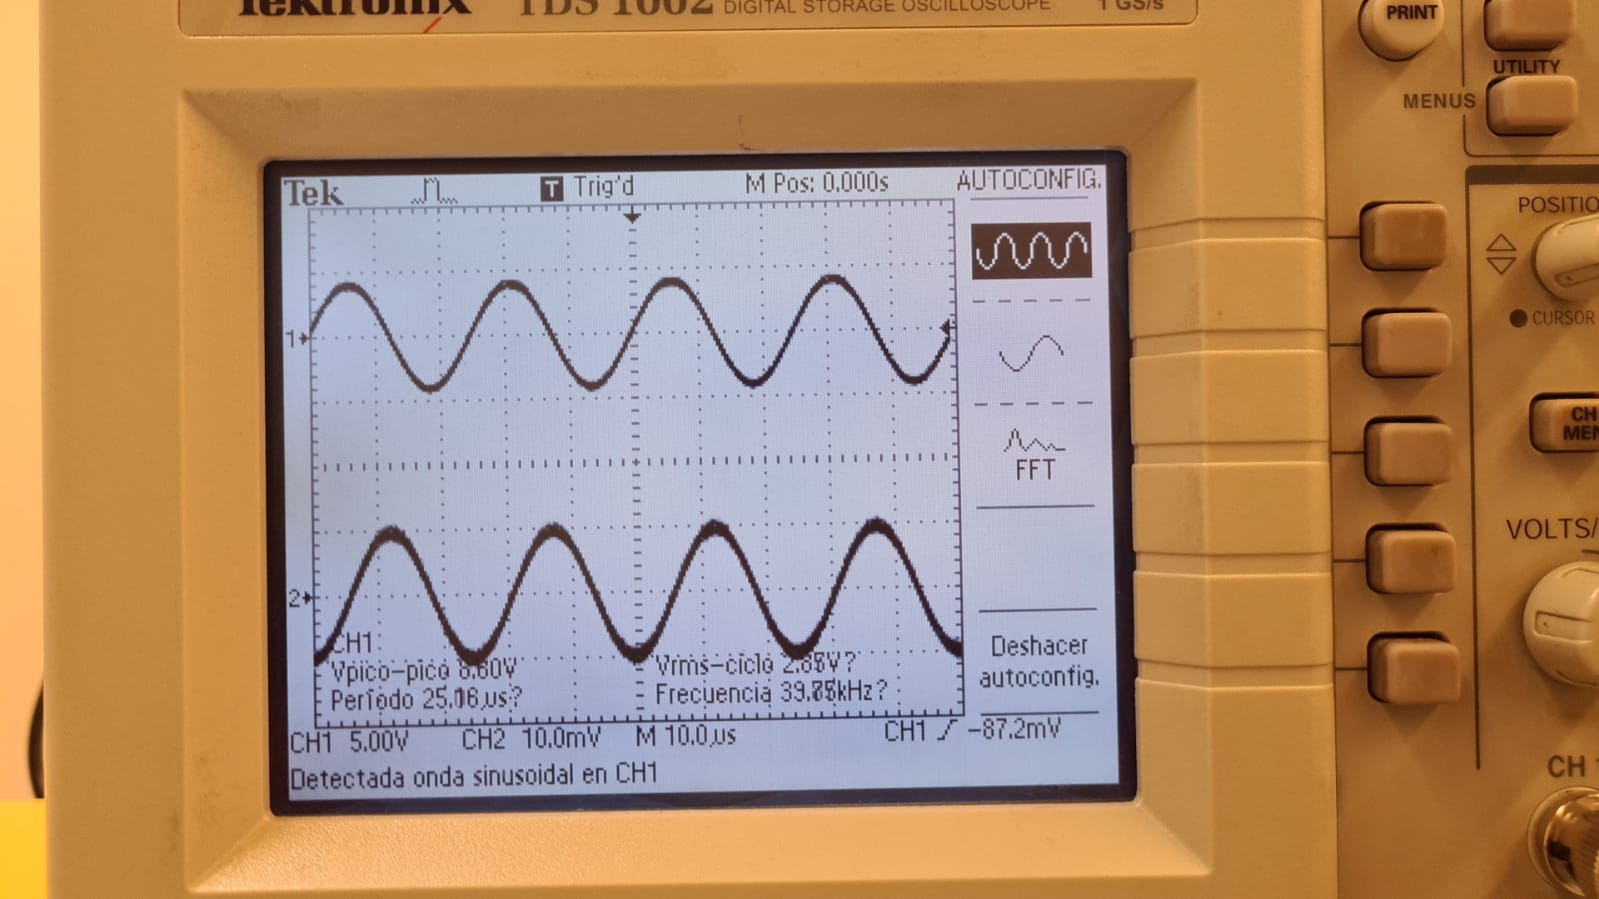
\includegraphics[width=100mm]{img_2_4.jpeg}
		\caption{Entrada i sortida del circuit total}
		\end{center}
	\end{figure}
	
	\textbf{Qüestió 6:}
	
	\begin{center}
		\scriptsize
		\begin{tabular}{ |c|c|c|c|c|c|c|c|c|c| } 
			\hline
			Freqüència & $100Hz$ & $1kHz$ & $10kHz$ & $25kHz$ & $40kHz$ & $75kHz$ & $100kHz$ & $500kHz$ & $1MHz$\\ \hline
			$V_{i1}$ & $20mV$ & $20mV$ & $20mV$ & $20mV$ & $20mV$ & $20mV$ & $20mV$ & $20mV$ & $20mV$\\ \hline
			$V_{o1}$ & $0V$ & $50mV$ & $0.2V$ & $1.4V$ & $4V$ & $5.6V$ & $6V$ & $400mV$ & $0$\\ \hline
			Guany & $0$ & $2.5$ & $10$ & $70$ & $200$ & $280$ & $300$ & $20$ & $0$\\ \hline
			Guany (dB) & $-$ & $7.9$ & $20$ & $36.9$ & $46$ & $48$ & $49.5$ & $26$ & $-$\\ \hline
		\end{tabular}
	\end{center}
	
	\textbf{Qüestió 7:} La tensió d'entrada per la que no hi ha distorció es $30mV$ ja que si fem $0.03\cdot 400 = 12 \approx V_{sat}$.

	\textbf{Qüestió 8:} Podem veure a les seguents imatges que el slew rate es igual a $SR = \frac{4-(-4)}{(250-(-500))\cdot 10^{-9}} = 10.6\frac{V}{\mu s}$
	
	\begin{figure}[H]
		\begin{center}
		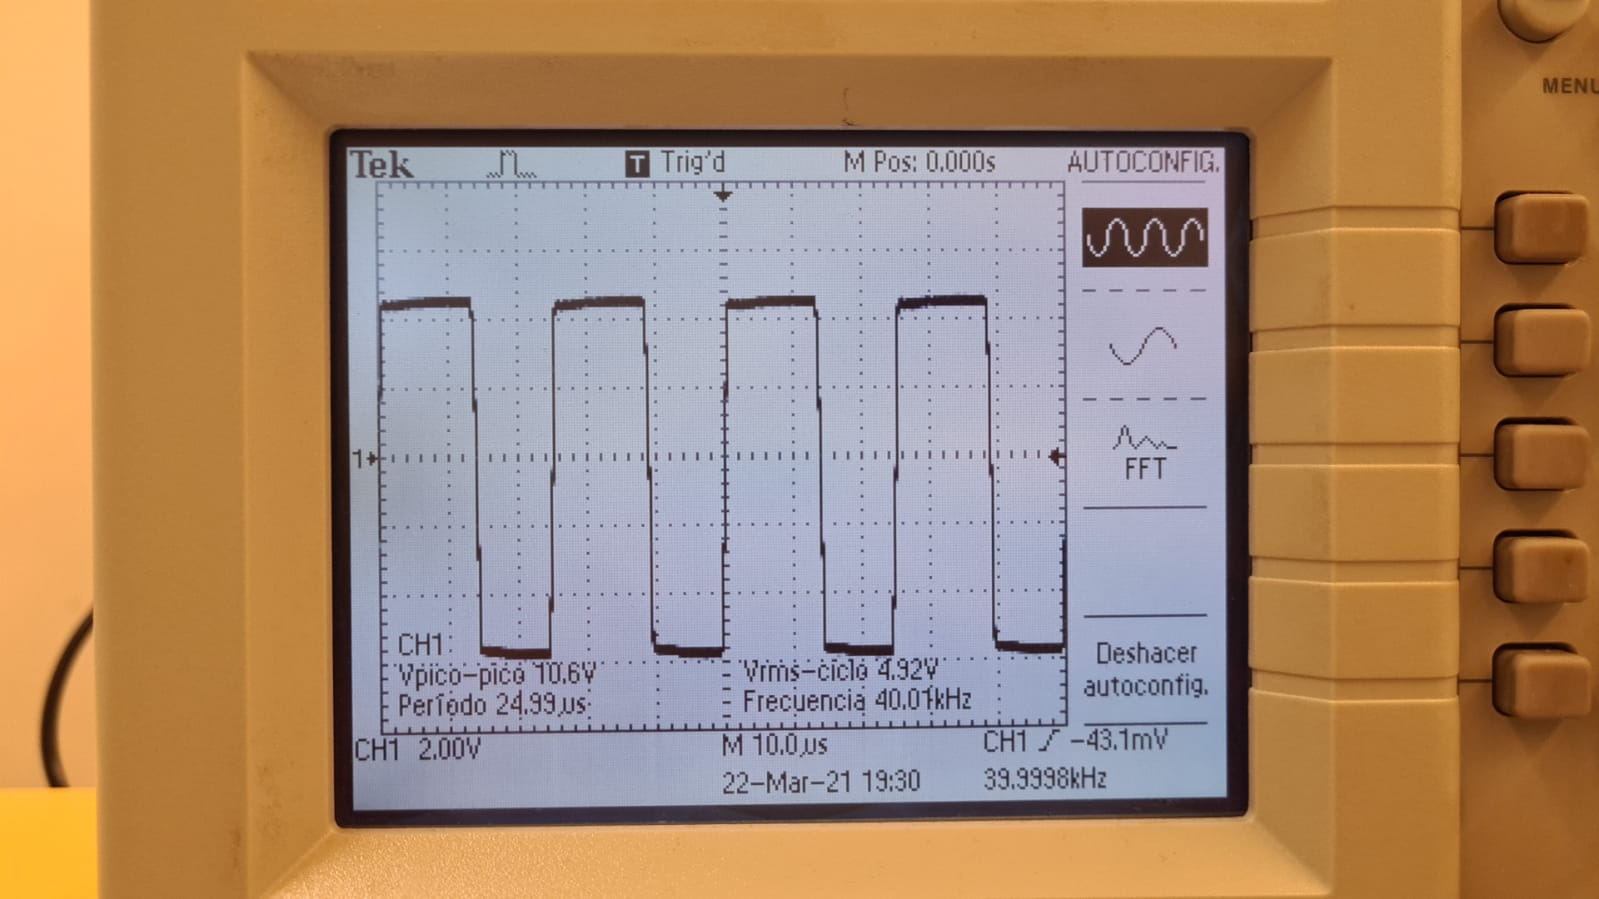
\includegraphics[width=100mm]{img_2_5.jpeg}
		\caption{Sortida del circuit amb entrada tensió elevada}
		\end{center}
	\end{figure}
	
	\begin{figure}[H]
		\begin{center}
		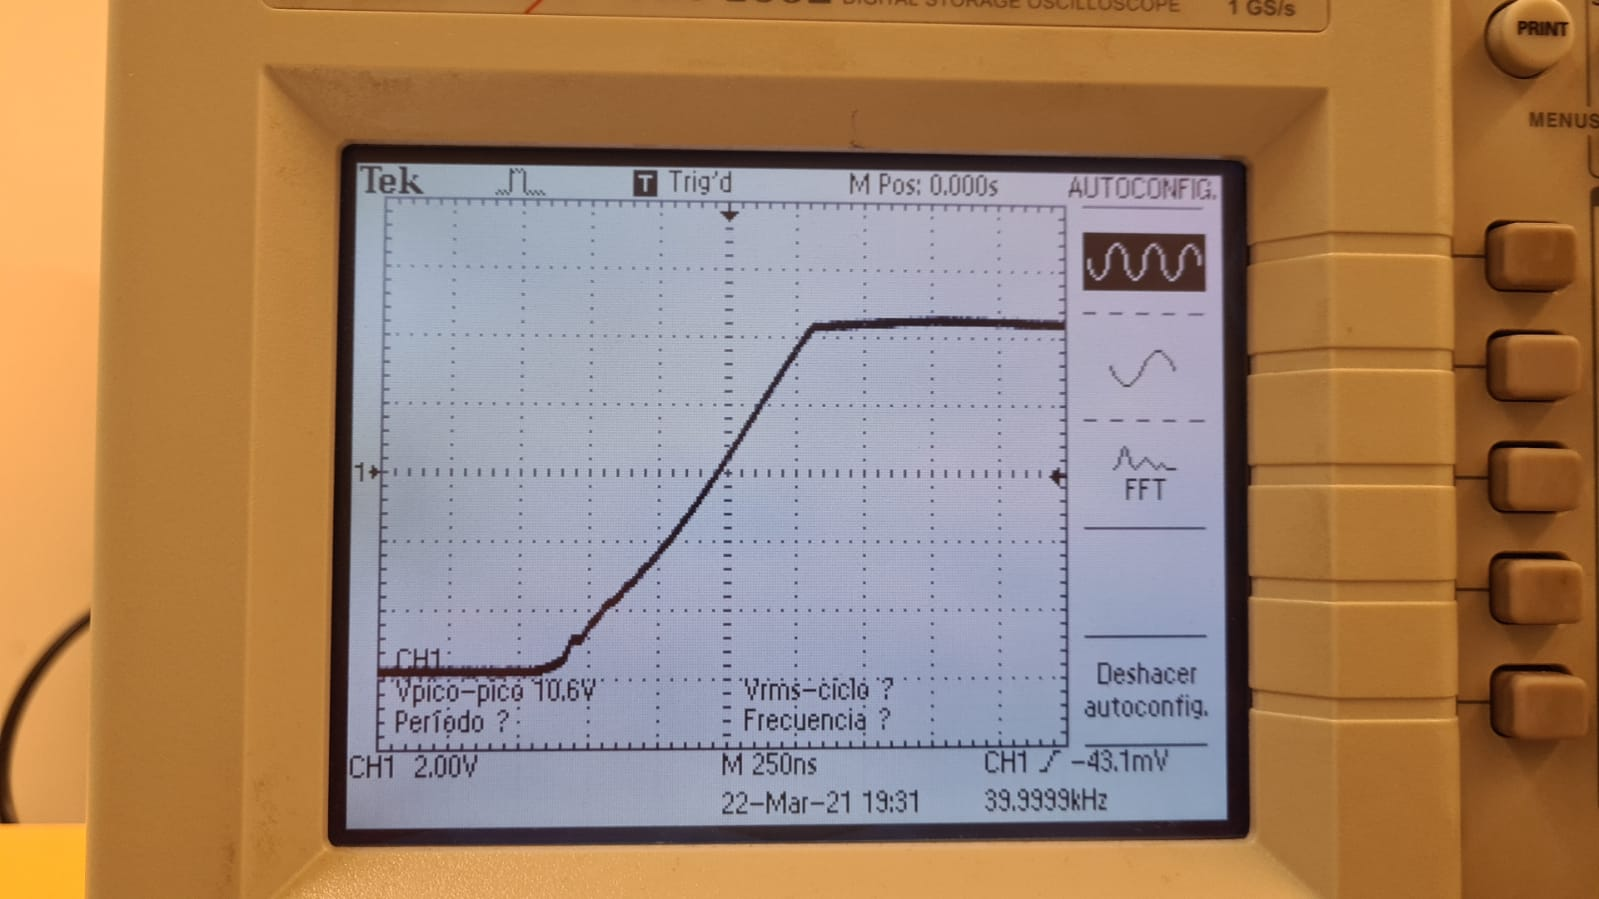
\includegraphics[width=100mm]{img_2_6.jpeg}
		\caption{Sortida del circuit amb entrada tensió elevada}
		\end{center}
	\end{figure}
	
\end{document}










